
% ************************************************************************
% CHAPTER 5: Subelement E5 - Electrical Principles
% ************************************************************************
\chapter{E5: Electrical Principles - The Heart of the Circuit!}

% ------------------------------------------------------------------------
% SECTION E5A: Resonance and Q
% ------------------------------------------------------------------------
\section{E5A: Resonance and Q - The Secrets of Circuits!}

\subsection*{Understanding the Basics}
Get ready to explore the electrical components behind radio and their properties! This section focuses on \textcolor{myblue}{\textbf{resonance and Q}}, an essential set of ideas in electrical circuits. You'll understand the meaning of \textcolor{myblue}{\textbf{resonant circuits}}, the fascinating state when components in the circuits react together to create an optimal condition. We'll also explore  \textcolor{myblue}{\textbf{series and parallel resonance}}, and how different configurations can impact a circuit's behavior and performance. Finally we will be introduced to  \textcolor{myblue}{\textbf{definitions and effects of Q}}, a measure of how efficiently a resonant circuit stores energy and  \textcolor{myblue}{\textbf{half-power bandwidth}} which provides you with the range of frequencies a filter is usable.

\mybox{mygreen}{
  \textbf{Fun Fact}: Did you know that the phenomenon of resonance is utilized across a vast variety of fields from musical instruments to laser technology and even to microwave ovens? This simple effect is one of the cornerstones of electrical engineering.
  }

\subsection*{Key Concepts for the Questions}
\begin{itemize}
    \item \textbf{Resonance:} The state when inductive and capacitive reactance in a circuit cancel each other out.
    \item \textbf{Series Resonance:} A state where a series RLC circuit exhibits a low impedance.
    \item \textbf{Parallel Resonance:} A state where a parallel RLC circuit exhibits a high impedance.
    \item \textbf{Q (Quality Factor):} A measure of how efficiently a resonant circuit stores energy.
    \item \textbf{Half-Power Bandwidth:} The frequency range where a resonant circuit's power response is reduced by 3 dB.
        \item  \textbf{Circulating current:} The reactive current in a parallel LC circuit.
\end{itemize}

\subsection*{Practice Questions}
\begin{enumerate}
  \item What can cause the voltage across reactances in a series RLC circuit to be higher than the voltage applied to the entire circuit?
    \begin{enumerate}
      \item \textbf{A. Resonance}
        \item  Capacitance
        \item  Low quality factor (Q)
        \item  Resistance
    \end{enumerate}
   \textcolor{myred}{Explanation:}
     At resonance the voltage across capacitive and inductive elements can be much higher than the input voltage.

   \item What is the resonant frequency of an RLC circuit if R is 22 ohms, L is 50 microhenries, and C is 40 picofarads?
     \begin{enumerate}
       \item  44.72 MHz
         \item  22.36 MHz
        \item \textbf{C. 3.56 MHz}
        \item  1.78 MHz
     \end{enumerate}
     \textcolor{myred}{Explanation:}
The resonant frequency $f_r$ of an RLC circuit is given by the formula:

$f_r = \frac{1}{2\pi\sqrt{LC}}$

Where:

\begin{itemize}
    \item $L$ is the inductance in henries (H)
    \item $C$ is the capacitance in farads (F)
\end{itemize}

Given:

\begin{itemize}
    \item $R = 22 \, \Omega$ (This value does not affect the resonant frequency)
    \item $L = 50 \, \mu\text{H} = 50 \times 10^{-6} \, \text{H}$
    \item $C = 40 \, \text{pF} = 40 \times 10^{-12} \, \text{F}$
\end{itemize}

Substituting the values into the formula:

\begin{align*}
f_r &= \frac{1}{2\pi\sqrt{(50 \times 10^{-6})(40 \times 10^{-12})}} \\
&= \frac{1}{2.8099 \times 10^{-7}} \\
&\approx 3.56 \times 10^6 \, \text{Hz}
\end{align*}

Therefore, the resonant frequency is approximately $3.56 \, \text{MHz}$.


  \item What is the magnitude of the impedance of a series RLC circuit at resonance?
       \begin{enumerate}
         \item  High, compared to the circuit resistance
        \item  Approximately equal to capacitive reactance
        \item  Approximately equal to inductive reactance
      \item \textbf{D. Approximately equal to circuit resistance}
    \end{enumerate}
       \textcolor{myred}{Explanation:}
         At resonance, capacitive and inductive reactance cancels each other, therefore the impedance will be equal to the resistive components of circuit.

    \item What is the magnitude of the impedance of a parallel RLC circuit at resonance?
    \begin{enumerate}
    \item \textbf{A. Approximately equal to circuit resistance}
     \item  Approximately equal to inductive reactance
       \item  Low compared to the circuit resistance
      \item  High compared to the circuit resistance
    \end{enumerate}
     \textcolor{myred}{Explanation:}
      In a parallel resonant circuit, impedance approaches the resistive components at resonance.
        
        \item What is the result of increasing the Q of an impedance-matching circuit?
    \begin{enumerate}
      \item \textbf{A. Matching bandwidth is decreased}
        \item  Matching bandwidth is increased
        \item  Losses increase
       \item  Harmonics increase
    \end{enumerate}
         \textcolor{myred}{Explanation:}
     A higher Q factor means smaller bandwidth for a matching circuit.

        \item What is the magnitude of the circulating current within the components of a parallel LC circuit at resonance?
       \begin{enumerate}
       \item  It is at a minimum
        \item \textbf{B. It is at a maximum}
       \item  It equals 1 divided by the quantity 2 times pi, times the square root of (inductance L multiplied by capacitance C)
         \item  It equals 2 times pi, times the square root of (inductance L multiplied by capacitance C)
        \end{enumerate}
        \textcolor{myred}{Explanation:}
    In parallel RLC circuits, at resonance the reactive current flow through inductive and capacitive components is maximum.
        
        \item What is the magnitude of the current at the input of a parallel RLC circuit at resonance?
       \begin{enumerate}
    \item \textbf{A. Minimum}
     \item  Maximum
        \item  R/L
     \item  L/R
    \end{enumerate}
   \textcolor{myred}{Explanation:}
       At resonance a parallel RLC circuit has maximum impedance, hence minimum current drawn by the source.
       
    \item What is the phase relationship between the current through and the voltage across a series resonant circuit at resonance?
     \begin{enumerate}
        \item  The voltage leads the current by 90 degrees
        \item  The current leads the voltage by 90 degrees
     \item \textbf{C. The voltage and current are in phase}
       \item  The voltage and current are 180 degrees out of phase
      \end{enumerate}
       \textcolor{myred}{Explanation:}
    At resonance of a series circuit voltage and current are in phase.

    \item How is the Q of an RLC parallel resonant circuit calculated?
      \begin{enumerate}
        \item \textbf{A. Reactance of either the inductance or capacitance divided by the resistance}
        \item  Reactance of either the inductance or capacitance multiplied by the resistance
       \item  Resistance divided by the reactance of either the inductance or capacitance
       \item  Reactance of the inductance multiplied by the reactance of the capacitance
        \end{enumerate}
       \textcolor{myred}{Explanation:}
        Q factor for a parallel resonant circuit is calculated as reactance divided by the resistance.

     \item What is the resonant frequency of an RLC circuit if R is 33 ohms, L is 50 microhenries, and C is 10 picofarads?
       \begin{enumerate}
        \item \textbf{A. 7.12 MHz}
       \item  23.5 kHz
        \item  7.12 kHz
         \item  23.5 MHz
       \end{enumerate}
       \textcolor{myred}{Explanation:}
   The resonant frequency is given by the formula $f = 1 / (2\pi * \sqrt{L*C})$, which is 7.12 MHz.

    \item What is the half-power bandwidth of a resonant circuit that has a resonant frequency of 7.1 MHz and a Q of 150?
    \begin{enumerate}
         \item  157.8 Hz
       \item  315.6 Hz
        \item \textbf{C. 47.3 kHz}
       \item  23.67 kHz
      \end{enumerate}
         \textcolor{myred}{Explanation:}
        The bandwidth of the resonant circuit can be calculated using f/Q which equals 47.3 kHz in this example.
    
     \item What is the half-power bandwidth of a resonant circuit that has a resonant frequency of 3.7 MHz and a Q of 118?
       \begin{enumerate}
     \item  436.6 kHz
     \item  218.3 kHz
     \item \textbf{C. 31.4 kHz}
         \item  15.7 kHz
       \end{enumerate}
    \textcolor{myred}{Explanation:}
       The bandwidth is equal to f/Q which is equal to 3.7 Mhz / 118 = 31.4 kHz

    \item What is an effect of increasing Q in a series resonant circuit?
      \begin{enumerate}
       \item  Fewer components are needed for the same performance
      \item  Parasitic effects are minimized
       \item \textbf{C. Internal voltages increase}
        \item  Phase shift can become uncontrolled
        \end{enumerate}
        \textcolor{myred}{Explanation:}
        Increasing the Q will increase the magnitude of voltage over its reactive component when reaching resonance.
\end{enumerate}

% ------------------------------------------------------------------------
% SECTION E5B: Time constants and phase relationships
% ------------------------------------------------------------------------
\section{E5B: Time Constants and Phase Relationships - The Timing of it All!}

\subsection*{Understanding the Basics}
Get ready to understand another important aspect of electrical circuits with \textcolor{myblue}{\textbf{time constants and phase relationships}}! In this section, we explore the fundamentals of \textcolor{myblue}{\textbf{RL and RC time constants}}, what it means for circuits with inductors and capacitors and how these elements can behave at different frequencies. Then we will learn about the concept of \textcolor{myblue}{\textbf{phase angle in reactive circuits and components}}, to understand how reactive components affect voltage-current relationship and delay, and understand the practical implication of these concepts with \textcolor{myblue}{\textbf{admittance and susceptance}}.

\mybox{mygreen}{
 \textbf{Fun Fact}: Did you know that time constants are what define how fast your flashlight starts glowing after you switch it on or how long it takes for the energy to leave your camera flash circuits after a flash?
  }

\subsection*{Key Concepts for the Questions}
\begin{itemize}
    \item \textbf{Time Constant:}  A measure of time it takes for a voltage or current in a circuit to decay by certain ratio, for either inductive (L/R) or capacitive (RC) circuits.
    \item \textbf{Phase Relationship:} How voltage and current of a signal are related in time with each other.
        \item \textbf{Admittance:}  The measure of how easily a circuit passes current, the inverse of impedance.
        \item  \textbf{Susceptance:} The imaginary component of admittance.
    \item \textbf{Impedance:} A measure of how much a circuit opposes current flow.
    \item \textbf{Reactance:} Opposition to the flow of alternating current due to capacitance or inductance.
     
\end{itemize}

\subsection*{Practice Questions}
\begin{enumerate}
   \item What is the term for the time required for the capacitor in an RC circuit to be charged to 63.2% of the applied voltage or to discharge to 36.8% of its initial voltage?
     \begin{enumerate}
       \item  An exponential rate of one
         \item \textbf{B. One time constant}
        \item  One exponential period
        \item  A time factor of one
      \end{enumerate}
    \textcolor{myred}{Explanation:}
    The time required for the capacitor to reach to 63.2% or fall to 36.8% of initial value is one time constant.

   \item What letter is commonly used to represent susceptance?
       \begin{enumerate}
         \item  G
         \item  X
        \item  Y
      \item \textbf{D. B}
       \end{enumerate}
     \textcolor{myred}{Explanation:}
    B is a common term used for susceptance, or imaginary part of admittance.

    \item How is impedance in polar form converted to an equivalent admittance?
      \begin{enumerate}
      \item  Take the reciprocal of the angle and change the sign of the magnitude
     \item \textbf{B. Take the reciprocal of the magnitude and change the sign of the angle}
      \item  Take the square root of the magnitude and add 180 degrees to the angle
        \item  Square the magnitude and subtract 90 degrees from the angle
        \end{enumerate}
    \textcolor{myred}{Explanation:}
    To convert impedance to admittance in polar form, one should take reciprocal of its magnitude and take negative of its angle.
       
      \item What is the time constant of a circuit having two 220-microfarad capacitors and two 1-megohm resistors, all in parallel?
      \begin{enumerate}
          \item  55 seconds
        \item  110 seconds
        \item  440 seconds
        \item \textbf{D. 220 seconds}
        \end{enumerate}
        \textcolor{myred}{Explanation:}
    Combined capacitor value in parallel is $220+220 = 440uF$, and resistors value is $1 M / 2 = 500K$, which gives $(440*10^{-6})* (500*10^3) = 220$ second time constant.
    
    \item What is the effect on the magnitude of pure reactance when it is converted to susceptance?
       \begin{enumerate}
       \item  It is unchanged
    \item  The sign is reversed
     \item  It is shifted by 90 degrees
       \item \textbf{D. It is replaced by its reciprocal}
      \end{enumerate}
        \textcolor{myred}{Explanation:}
         Susceptance is the reciprocal of reactance.
        
   \item What is susceptance?
        \begin{enumerate}
         \item  The magnetic impedance of a circuit
      \item  The ratio of magnetic field to electric field
         \item \textbf{C. The imaginary part of admittance}
      \item  A measure of the efficiency of a transformer
    \end{enumerate}
       \textcolor{myred}{Explanation:}
     Susceptance is the imaginary portion of admittance, which includes capacitive and inductive properties of circuit.

  \item What is the phase angle between the voltage across and the current through a series RLC circuit if XC is 500 ohms, R is 1 kilohm, and XL is 250 ohms?
    \begin{enumerate}
       \item  68.2 degrees with the voltage leading the current
       \item  14.0 degrees with the voltage leading the current
       \item \textbf{C. 14.0 degrees with the voltage lagging the current}
         \item  68.2 degrees with the voltage lagging the current
        \end{enumerate}
     \textcolor{myred}{Explanation:}
      The phase angle can be calculated with arctan[(XL-XC)/R], in this case arctan[(250-500)/1000] which is around 14 degrees, where current is lagging the voltage.

      \item What is the phase angle between the voltage across and the current through a series RLC circuit if XC is 300 ohms, R is 100 ohms, and XL is 100 ohms?
       \begin{enumerate}
       \item \textbf{A. 63 degrees with the voltage lagging the current}
         \item  63 degrees with the voltage leading the current
        \item  27 degrees with the voltage leading the current
      \item  27 degrees with the voltage lagging the current
        \end{enumerate}
        \textcolor{myred}{Explanation:}
          The phase angle can be calculated with arctan[(XL-XC)/R], in this case arctan[(100-300)/100] which is approximately 63 degrees, with current lagging the voltage.

    \item What is the relationship between the AC current through a capacitor and the voltage across a capacitor?
       \begin{enumerate}
      \item  Voltage and current are in phase
       \item  Voltage and current are 180 degrees out of phase
      \item  Voltage leads current by 90 degrees
      \item \textbf{D. Current leads voltage by 90 degrees}
     \end{enumerate}
     \textcolor{myred}{Explanation:}
    In a capacitor, current leads the voltage by 90 degrees.
      
      \item What is the relationship between the AC current through an inductor and the voltage across an inductor?
       \begin{enumerate}
         \item \textbf{A. Voltage leads current by 90 degrees}
         \item  Current leads voltage by 90 degrees
        \item  Voltage and current are 180 degrees out of phase
      \item  Voltage and current are in phase
        \end{enumerate}
    \textcolor{myred}{Explanation:}
     In an inductor, voltage leads the current by 90 degrees.

   \item What is the phase angle between the voltage across and the current through a series RLC circuit if XC is 25 ohms, R is 100 ohms, and XL is 75 ohms?
    \begin{enumerate}
        \item  27 degrees with the voltage lagging the current
        \item \textbf{B. 27 degrees with the voltage leading the current}
      \item  63 degrees with the voltage lagging the current
       \item  63 degrees with the voltage leading the current
     \end{enumerate}
       \textcolor{myred}{Explanation:}
        The phase angle can be calculated with arctan[(XL-XC)/R], in this case arctan[(75-25)/100] which is around 27 degrees, where voltage is leading the current.

  \item What is admittance?
   \begin{enumerate}
    \item \textbf{A. The inverse of impedance}
        \item  The term for the gain of a field effect transistor
       \item  The inverse of reactance
      \item  The term for the on-impedance of a field effect transistor
   \end{enumerate}
      \textcolor{myred}{Explanation:}
      Admittance is the reciprocal of impedance and measured in Siemens (S).
\end{enumerate}

% ------------------------------------------------------------------------
% SECTION E5C: Coordinate Systems and Phasors
% ------------------------------------------------------------------------
\section{E5C: Coordinate Systems and Phasors - Mapping Out the Electrics!}

\subsection*{Understanding the Basics}
Let’s explore the exciting topic of how we can visualize electrical quantities with \textcolor{myblue}{\textbf{coordinate systems and phasors}}! This section introduces \textcolor{myblue}{\textbf{rectangular coordinates}} that allows representing complex numbers as X+jY in a graph, as well as \textcolor{myblue}{\textbf{polar coordinates}} using magnitude and phase angle.  Then we will be introduced to \textcolor{myblue}{\textbf{phasors}}, which help in calculating ac values by looking at them as vector representation and then finally we'll see how to make use of \textcolor{myblue}{\textbf{logarithmic axes}} to better understand wide-range values in circuit analysis.

\mybox{mygreen}{
  \textbf{Fun Fact}: Did you know that representing electrical quantities as vectors or complex numbers allows engineers and hams to design and analyze complex circuits more easily?
  }
\subsection*{Key Concepts for the Questions}
\begin{itemize}
    \item \textbf{Rectangular Coordinates:} Representation of a complex number in form of a + jb.
        \item \textbf{Polar Coordinates:} Representation of a complex number in magnitude and phase angle.
    \item \textbf{Phasor:} A rotating vector representation of a sinusoidal signal.
        \item \textbf{Logarithmic Axis:} A scale used in graphs that helps to better represent wide ranges of values.
     \item \textbf{Admittance:}  The reciprocal of impedance, in polar form.
      \item \textbf{Reactance:}  Opposition to alternating current, in polar form.

\end{itemize}

\subsection*{Practice Questions}
\begin{enumerate}
    \item Which of the following represents pure capacitive reactance of 100 ohms in rectangular notation?
    \begin{enumerate}
     \item \textbf{A. 0 - j100}
       \item  0 + j100
        \item  100 - j0
      \item  100 + j0
    \end{enumerate}
     \textcolor{myred}{Explanation:}
    In rectangular form, purely capacitive reactance is expressed as a negative imaginary value such as  0-j100.

      \item How are impedances described in polar coordinates?
       \begin{enumerate}
    \item  By X and R values
         \item  By real and imaginary parts
      \item \textbf{C. By magnitude and phase angle}
       \item  By Y and G values
    \end{enumerate}
    \textcolor{myred}{Explanation:}
      In polar coordinates, the complex number is represented with magnitude and phase angle.
       
  \item Which of the following represents a pure inductive reactance in polar coordinates?
    \begin{enumerate}
    \item  A positive 45 degree phase angle
        \item  A negative 45 degree phase angle
        \item \textbf{C. A positive 90 degree phase angle}
        \item  A negative 90 degree phase angle
     \end{enumerate}
     \textcolor{myred}{Explanation:}
      Inductive reactance is expressed as positive 90 degree phase angle in polar form.

    \item What type of Y-axis scale is most often used for graphs of circuit frequency response?
    \begin{enumerate}
    \item  Linear
        \item  Scatter
     \item  Random
      \item \textbf{D. Logarithmic}
    \end{enumerate}
       \textcolor{myred}{Explanation:}
       Logarithmic Y-axis helps better visualize large variations in the magnitude response of a circuit over frequency.
        
      \item What kind of diagram is used to show the phase relationship between impedances at a given frequency?
       \begin{enumerate}
         \item  Venn diagram
        \item  Near field diagram
         \item \textbf{C. Phasor diagram}
      \item  Far field diagram
      \end{enumerate}
         \textcolor{myred}{Explanation:}
         Phasor diagram is used for representing phase and magnitude of circuit elements with vectors.
          
    \item What does the impedance 50 - j25 ohms represent?
      \begin{enumerate}
      \item  50 ohms resistance in series with 25 ohms inductive reactance
         \item \textbf{B. 50 ohms resistance in series with 25 ohms capacitive reactance}
        \item  25 ohms resistance in series with 50 ohms inductive reactance
         \item  25 ohms resistance in series with 50 ohms capacitive reactance
     \end{enumerate}
   \textcolor{myred}{Explanation:}
   In the rectangular coordinate, a negative sign at the imaginary part implies a capacitive reactance.
        
    \item Where is the impedance of a pure resistance plotted on rectangular coordinates?
       \begin{enumerate}
         \item  On the vertical axis
          \item  On a line through the origin, slanted at 45 degrees
        \item  On a horizontal line, offset vertically above the horizontal axis
       \item \textbf{D. On the horizontal axis}
       \end{enumerate}
       \textcolor{myred}{Explanation:}
      Purely resistive values will be located on X axis of the rectangular coordinate.

    \item What coordinate system is often used to display the phase angle of a circuit containing resistance, inductive, and/or capacitive reactance?
     \begin{enumerate}
      \item  Maidenhead grid
        \item  Faraday grid
      \item  Elliptical coordinates
      \item \textbf{D. Polar coordinates}
      \end{enumerate}
     \textcolor{myred}{Explanation:}
        Polar coordinates with magnitude and phase angle are the most common way for graphically displaying both components of the impedance.
   
    \item When using rectangular coordinates to graph the impedance of a circuit, what do the axes represent?
       \begin{enumerate}
       \item \textbf{A. The X axis represents the resistive component, and the Y axis represents the reactive component}
       \item  The X axis represents the reactive component, and the Y axis represents the resistive component
      \item  The X axis represents the phase angle, and the Y axis represents the magnitude
        \item  The X axis represents the magnitude, and the Y axis represents the phase angle
       \end{enumerate}
     \textcolor{myred}{Explanation:}
    In a rectangular coordinate, x axis represents the resistive value and Y axis represents the reactive value.
    
        
       \item Which point on Figure E5-1 best represents the impedance of a series circuit consisting of a 400-ohm resistor and a 38-picofarad capacitor at 14 MHz? 
           
           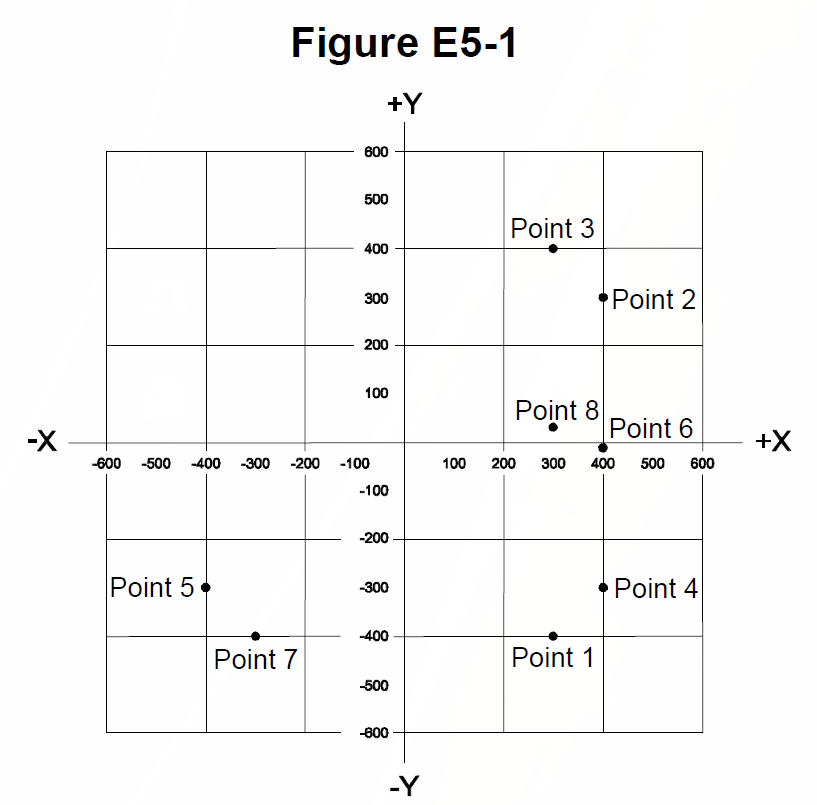
\includegraphics[width=0.8\textwidth]{images/e5-1.png}

         \begin{enumerate}
       \item  Point 2
       \item \textbf{B. Point 4}
        \item  Point 5
       \item  Point 6
        \end{enumerate}
      \textcolor{myred}{Explanation:}
       At 14MHz, 38 pF capacitor produces an impedance of around 300 Ohms and thus will result in 400-j300 value. Point 4 is closest to that.

     \item Which point in Figure E5-1 best represents the impedance of a series circuit consisting of a 300-ohm resistor and an 18-microhenry inductor at 3.505 MHz?
       \begin{enumerate}
       \item  Point 1
        \item \textbf{B. Point 3}
         \item  Point 7
        \item  Point 8
        \end{enumerate}
        \textcolor{myred}{Explanation:}
    At 3.505 MHz, 18uH inductor produces a impedance close to j400 thus the combined impedance should be 300+j400 which point 3 is closest to.
        
      \item Which point on Figure E5-1 best represents the impedance of a series circuit consisting of a 300-ohm resistor and a 19-picofarad capacitor at 21.200 MHz?
       \begin{enumerate}
    \item \textbf{A. Point 1}
       \item  Point 3
       \item  Point 7
       \item  Point 8
        \end{enumerate}
   \textcolor{myred}{Explanation:}
    At 21.2 MHz 19 pF capacitor generates a -j400 impedance. Combining with 300 Ohm resistor will result in 300-j400 ohms which is represented best by point 1.
\end{enumerate}

% ------------------------------------------------------------------------
% SECTION E5D: RF Effects in Components and Circuits
% ------------------------------------------------------------------------
\section{E5D: RF Effects in Components and Circuits -  When RF Gets Real!}
\subsection*{Understanding the Basics}
Time to learn about \textcolor{myblue}{\textbf{RF effects in components and circuits}}! You will explore the details of \textcolor{myblue}{\textbf{skin effect}}, that describes how RF current flows more on the surface of a conductor. We will then study the distinction between  \textcolor{myblue}{\textbf{real and reactive power}} and understand how these different power types are related to the circuit operation. Finally, we'll touch upon the concept of  \textcolor{myblue}{\textbf{electrical length of conductors}}, which matters for signal transmissions, specifically at higher frequencies.

\mybox{mygreen}{
   \textbf{Fun Fact}: Did you know that a small electrical wire can have a different effective electrical length depending on the frequency it is used for, even though the physical length is always the same! This can drastically change the impedance of a circuit in high frequency RF design!
  }
\subsection*{Key Concepts for the Questions}
\begin{itemize}
    \item \textbf{Skin Effect:} The tendency of high-frequency current to flow on the outer layers of a conductor.
        \item \textbf{Real Power:} Power that is consumed in a circuit.
    \item \textbf{Reactive Power:} The power oscillating back and forth in reactive components.
     \item \textbf{Electrical Length:}  The length of a conductor with respect to signal’s wavelength, not physical dimension.
         \item \textbf{Reactive Power:} The energy that flows into and out of reactive components and does not get converted into heat.
        
\end{itemize}

\subsection*{Practice Questions}
\begin{enumerate}
    \item What is the result of conductor skin effect?
        \begin{enumerate}
        \item \textbf{A. Resistance increases as frequency increases because RF current flows closer to the surface}
        \item  Resistance decreases as frequency increases because electron mobility increases
         \item  Resistance increases as temperature increases because of the change in thermal coefficient
          \item  Resistance decreases as temperature increases because of the change in thermal coefficient
      \end{enumerate}
     \textcolor{myred}{Explanation:}
       Skin effect results in reduction in the effective cross sectional area for current flow, hence increase in resistance.

   \item Why is it important to keep lead lengths short for components used in circuits for VHF and above?
       \begin{enumerate}
        \item  To increase the thermal time constant
        \item \textbf{B. To minimize inductive reactance}
        \item  To maintain component lifetime
        \item  All these choices are correct
        \end{enumerate}
       \textcolor{myred}{Explanation:}
         A conductor acts like an inductor, its impedance increases by length and especially at higher frequencies, limiting its use in circuits.
         
    \item What is the phase relationship between current and voltage for reactive power?
       \begin{enumerate}
          \item  They are out of phase
          \item  They are in phase
       \item \textbf{C. They are 90 degrees out of phase}
     \item  They are 45 degrees out of phase
        \end{enumerate}
     \textcolor{myred}{Explanation:}
      Reactive power only oscillates in reactive elements.
       
    \item Why are short connections used at microwave frequencies?
      \begin{enumerate}
        \item  To increase neutralizing resistance
       \item \textbf{B. To reduce phase shift along the connection}
    \item  To increase compensating capacitance
     \item  To reduce noise figure
      \end{enumerate}
       \textcolor{myred}{Explanation:}
    At higher frequencies short connections reduce parasitic impedance changes and phase differences in different parts of a circuit, which can cause problems with proper performance.

   \item What parasitic characteristic causes electrolytic capacitors to be unsuitable for use at RF?
     \begin{enumerate}
      \item  Skin effect
      \item  Shunt capacitance
     \item \textbf{C. Inductance}
     \item  Dielectric leakage
     \end{enumerate}
    \textcolor{myred}{Explanation:}
    Electrolytic capacitors, due to their construction, always have parasitic inductance, rendering them ineffective in RF applications.
       
    \item What parasitic characteristic creates an inductor's self-resonance?
       \begin{enumerate}
       \item  Skin effect
       \item  Dielectric loss
       \item  Coupling
       \item \textbf{D. Inter-turn capacitance}
      \end{enumerate}
        \textcolor{myred}{Explanation:}
       Inter turn capacitance creates parasitic self-resonance in inductors.

      \item What combines to create the self-resonance of a component?
        \begin{enumerate}
       \item  The component's resistance and reactance
    \item \textbf{B. The component's nominal and parasitic reactance}
       \item  The component's inductance and capacitance
       \item  The component's electrical length and impedance
       \end{enumerate}
         \textcolor{myred}{Explanation:}
       A component's self resonance is defined by parasitic and normal reactances that form its components.
        
      \item What is the primary cause of loss in film capacitors at RF?
      \begin{enumerate}
     \item  Inductance
       \item \textbf{B. Dielectric loss}
       \item  Self-discharge
       \item  Skin effect
        \end{enumerate}
       \textcolor{myred}{Explanation:}
        At higher frequencies, loss is caused by dielectric properties of the film capacitor material.
        
  \item What happens to reactive power in ideal inductors and capacitors?
    \begin{enumerate}
      \item  It is dissipated as heat in the circuit
         \item \textbf{B. Energy is stored in magnetic or electric fields, but power is not dissipated}
         \item  It is canceled by Coulomb forces in the capacitor and inductor
       \item  It is dissipated in the formation of inductive and capacitive fields
       \end{enumerate}
     \textcolor{myred}{Explanation:}
        Reactive power, flows back and forth and ideally it is not converted into heat, but stored in the reactive components.
   
   \item As a conductor's diameter increases, what is the effect on its electrical length?
      \begin{enumerate}
      \item  Thickness has no effect on electrical length
        \item  It varies randomly
        \item  It decreases
       \item \textbf{D. It increases}
        \end{enumerate}
         \textcolor{myred}{Explanation:}
    As conductor diameter increases, its electrical length increases.
    
    \item How much real power is consumed in a circuit consisting of a 100-ohm resistor in series with a 100-ohm inductive reactance drawing 1 ampere?
        \begin{enumerate}
         \item  70.7 watts
         \item \textbf{B. 100 watts}
         \item  141.4 watts
         \item  200 watts
        \end{enumerate}
         \textcolor{myred}{Explanation:}
     Only the resistor dissipates real power. Real power is calculated by $I^2*R$, which is $1*1*100 = 100W$.
        
        \item What is reactive power?
        \begin{enumerate}
    \item  Power consumed in circuit Q
       \item  Power consumed by an inductor's wire resistance
     \item  The power consumed in inductors and capacitors
         \item \textbf{D. Wattless, nonproductive power}
       \end{enumerate}
    \textcolor{myred}{Explanation:}
         Reactive power is power oscillating back and forth, without conversion to work or heat.
\end{enumerate}
